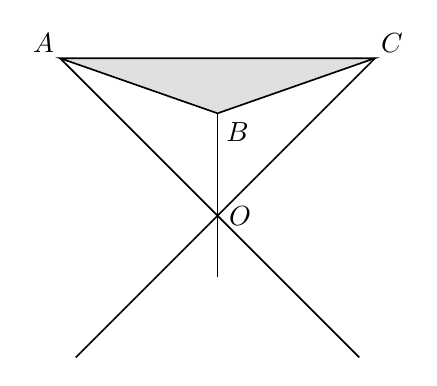
\begin{tikzpicture}[x=1cm,y=1cm,font=\normalsize,
  geometry edge/.style={solid,line width=.6pt,draw=black},
  geometry label/.style={font=\normalsize,inner sep=2pt}]
% Schematic stool projection: triangle ABC on top, three legs concurrent at O
\coordinate (A) at (0,4);
\coordinate (C) at (4,4);
\coordinate (B) at (2,3.3);
\coordinate (O) at (2,2);
\coordinate (Ap) at (3.8,0.2);
\coordinate (Cp) at (0.2,0.2);
\coordinate (Bp) at (2,1.22);
\fill[black!12] (A)--(B)--(C)--cycle;
\draw[geometry edge] (A)--(C)--(B)--cycle;
\draw[geometry edge] (A)--(Ap);
\draw[geometry edge] (C)--(Cp);
\draw[geometry edge] (B)--(Bp);
\node[geometry label,above left] at (A) {$A$};
\node[geometry label,above right] at (C) {$C$};
\node[below right,inner sep=3pt] at (B) {$B$};
\node[right,inner sep=4pt] at (O) {$O$};
\end{tikzpicture}
